%=============================================================
Una prima via per controllare il sistema, è rappresentata dalla modalità manuale:
essa permette di gestire direttamente, in \emph{tempo reale}, la posizioni di ognuno dei 6 giunti del manipolatore IRB 120, ad una velocità di movimento però limitata per questioni di sicurezza.

Ciò è possibile grazie alla \emph{Flex pendant} \label{text:FlexPendant}, in alcuni casi indicata anche come \emph{TPU} o Teach Pendant Unit, la quale è utilizzata per eseguire molte delle operazioni correlate al funzionamento di un sistema robotico: esecuzione dei programmi, movimentazione manuale del manipolatore, modifica di programmi a bordo del controllore ecc\dots\cite{ABB:Web_FlexPendant}.

Per capire quali sono gli utilizzi principali in cui la Flex Pendant ricopre un ruolo di primaria importanza, andiamo ad analizzare quelle che sono le principali parti \emph{fisiche} componenti l'unità stessa (figura~\vref{fig:FlexPendantParti}).
\begin{figure}[h]
	\centering
	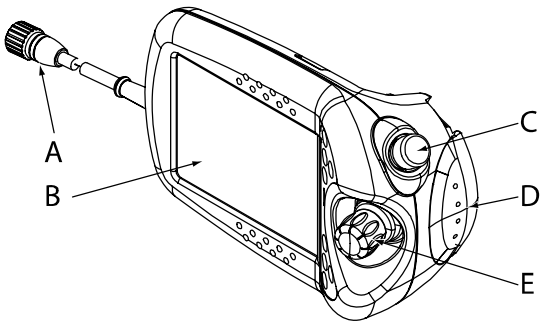
\includegraphics[width=0.5\textwidth]{Immagini/MainPart_TeachPendant}
	\caption{Componenti principali della Flex Pendant}{\cite{ABB:Web_FlexPendant}}
	\label{fig:FlexPendantParti}
\end{figure}

I componenti principali della Flex Pendant sono:
\begin{itemize}
	\item[A: ] Connettore
	\item[B: ] Touch screen
	\item[C: ] Pulsante di arresto di emergenza
	\item[D: ] Dispositivo di attivazione
	\item[E: ] Joystick
\end{itemize}

Si vede come, la Flex Pendant, sia decisamente adatta per la movimentazione manuale tramite il pratico joystick: esso permette di gestire contemporaneamente la movimentazione di tre assi per volta, unitamente ad un supporto visivo a schermo, che consente di configurare la movimentazione.
\begin{figure}[h]
	\centering
	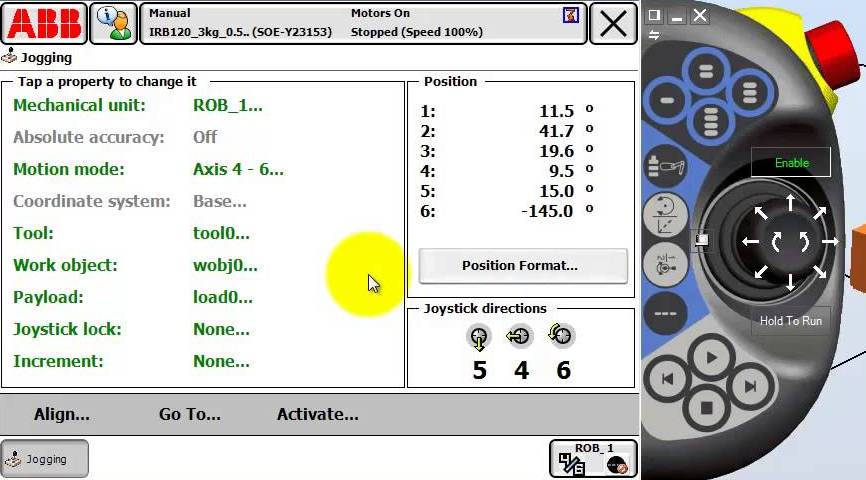
\includegraphics[width=0.5\textwidth]{Immagini/DisplayTPU_ManualJog}
	\caption{Schermata di controllo della movimentazione manuale tramite joystick}
	%[Immagine presa dal sito https://www.youtube.com/watch?v=cRQUxkt73is in data 25/02/18] 
	\label{fig:DisplayFlexPendant}
\end{figure}

Come si può vedere in figura~\vref{fig:DisplayFlexPendant}, la Flex Pendant permette di visualizzare, in tempo reale, la posizione dei 6 giunti, tramite una visualizzazione che può essere impostata in gradi oppure in radianti, fornendo anche la possibilità di gestire la movimentazione giunto per giunto oppure in maniera lineare o alternativamente secondo una tecnica circolare, a seconda delle esigenze specifiche. 

Si può inoltre andare a selezionare quale terna di giunti (1-2-3 o 4-5-6) sono oggetto di movimentazione tramite jog manuale, quale manipolatore, nei sistemi multimove, si vuole gestire potendo visualizzare allo stesso tempo anche i sistemi di coordinate alle quali il moto si riferisce.
Questa modalità di utilizzo rappresenta sicuramente un modo rapido e sicuro per gestire in maniera diretta la posizione del manipolatore: a livello di prestazioni e di funzionalità, come si può ben capire, è decisamente però una modalità molto limitante, al solo scopo dimostrativo e/o di setting-up.
%=============================================================